%!TEX root = ../template.tex
%%%%%%%%%%%%%%%%%%%%%%%%%%%%%%%%%%%%%%%%%%%%%%%%%%%%%%%%%%%%%%%%%%%%
%% chapter4.tex
%% NOVA thesis document file
%%
%% Chapter with a short latex tutorial and examples
%%%%%%%%%%%%%%%%%%%%%%%%%%%%%%%%%%%%%%%%%%%%%%%%%%%%%%%%%%%%%%%%%%%%

\typeout{NT FILE chapter4.tex}%

\chapter{MOBs}
\label{cha:mobs}

\section{Overview}
\label{sub:overview}

MOBs standing for Modular Blockchain Simulator is divided into two main components,
the simulator a and the graphical user interface, we will look into them seperatly.

\subsection{Simulator}
\label{subsec:simulator}

The simulator makes use of OCaml's \textit{modules} and \textit{functors} to
provide modularity and extensibility. MOBs adopts a \textit{Discrete-Event Simulation Model}
making the state of the system only change in discrete points in time when events occur.
These events are stored in a queue ordered with two main values:
\begin{itemize}
  \item \textbf{Timestamp:} This value dictates the order in which the events are
stored in the queue and is based on the simulator's internal clock. When getting
a new event the simulator will fetch from the queue the one with the smallest timestamp
and move its internal clock to match that event's timestamp.
  \item \textbf{Target:} The entity that should process this event.
\end{itemize}
Events are fetched from the queue until no more events remain or a predefined
stopping condition is reached.

\begin{figure}[h]
	\centering
	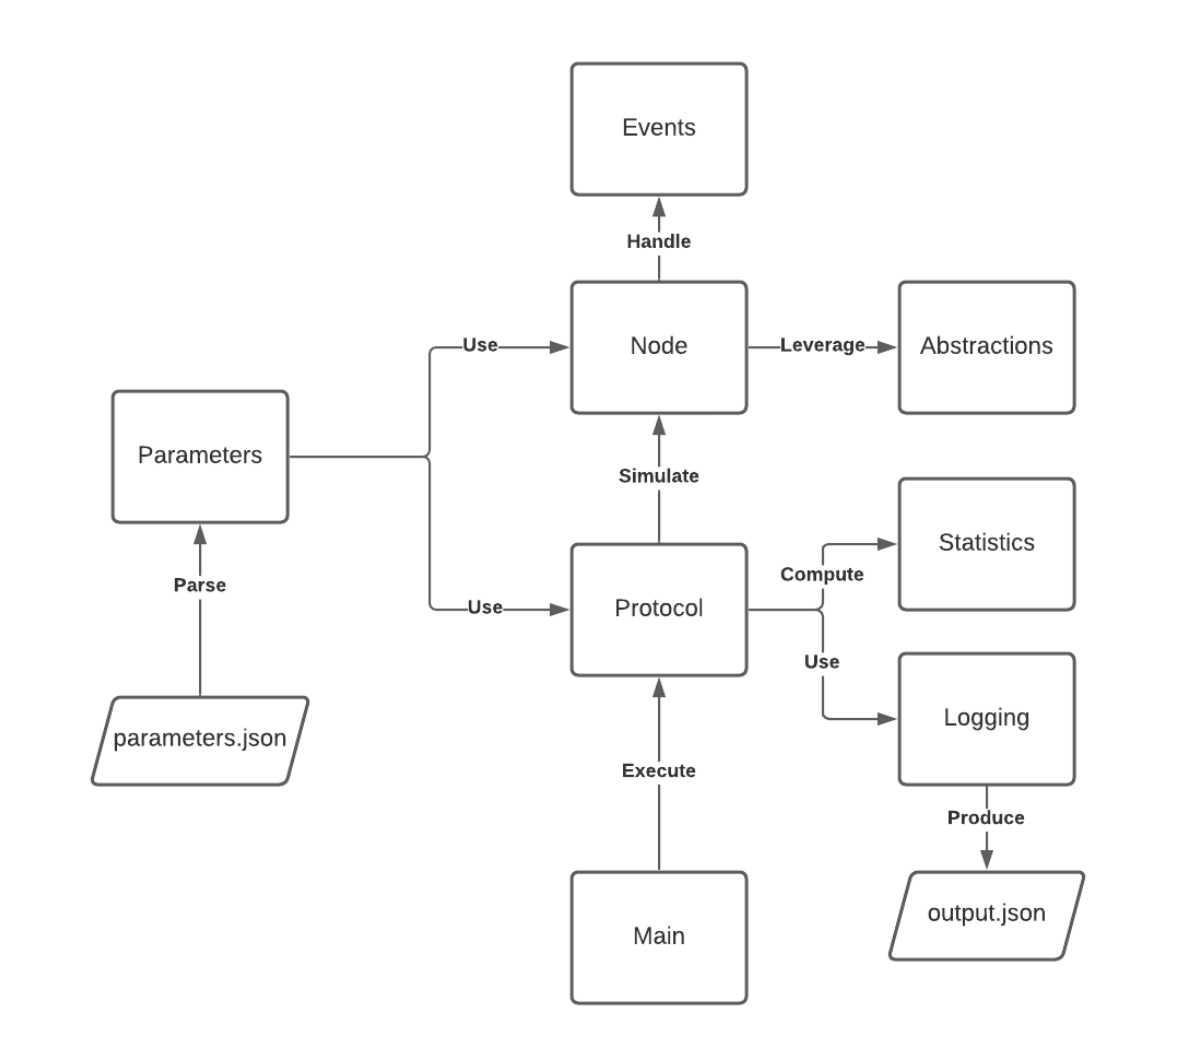
\includegraphics[width=4.5in, angle =0]{modules_mobs}
	\caption{Ilustration of top-level module interactions}
	\label{fig:modules_mobs}
\end{figure}

The simulator is built in a module based architecture, Figure \ref{fig:modules_mobs} illustrates
how the different modules interact. These modules are:
\begin{itemize}
  \item \textbf{Main:} Entry point for the simulator, manages the execution of
protocols.
  \item \textbf{Protocol:} Top-level loop of the simulation, initializes the different
nodes, network topology, event queue and performs event handling and delegation.
  \item \textbf{Node:} This is a user defined module that describes the behaviour
of an entity in the simulated protocol.
  \item \textbf{Abstractions:} This module provides primitives to aid in the
development of new simulation such as proof of stake sortation, proof of work mining,
timers, alarms and message exchanges.
  \item \textbf{Statistics and Logging:}  Extract metrics and values from the execution
to be processed by the GUI.
\end{itemize}

\subsection{Graphical User Interface}
\label{subsec:grafical_user_interface}

The graphical user interface was implemented in NodeJs, Vue3 and ElectronJS.
The choice for web technologies enables the future deployement of simulator as
a web application. The GUI was developed with the goal of allowing the users
to use it with their own custom simulators as long as the following conditions are met:

\begin{enumerate}
  \item The simulator uses a parameters.json as an input with three categories,
General, Network and Protocol, the actual parameters inside each category are user defined.
  \item The output of the simulator produces log with two top-level entries, kind and content.
Kind can be one of ten values, each with their specific content, \textit{parameters, 
add-node, add-link, flow-message, add-block, node-committee, node-proposer, create-block,
statistics} and \textit{per-node-statistics}.
\end{enumerate}

The GUI is composed of 4 pages, described in the following sections.

\subsubsection{Parametrization}
\label{subsubsec:parametrization}

\begin{figure}[h]
	\centering
	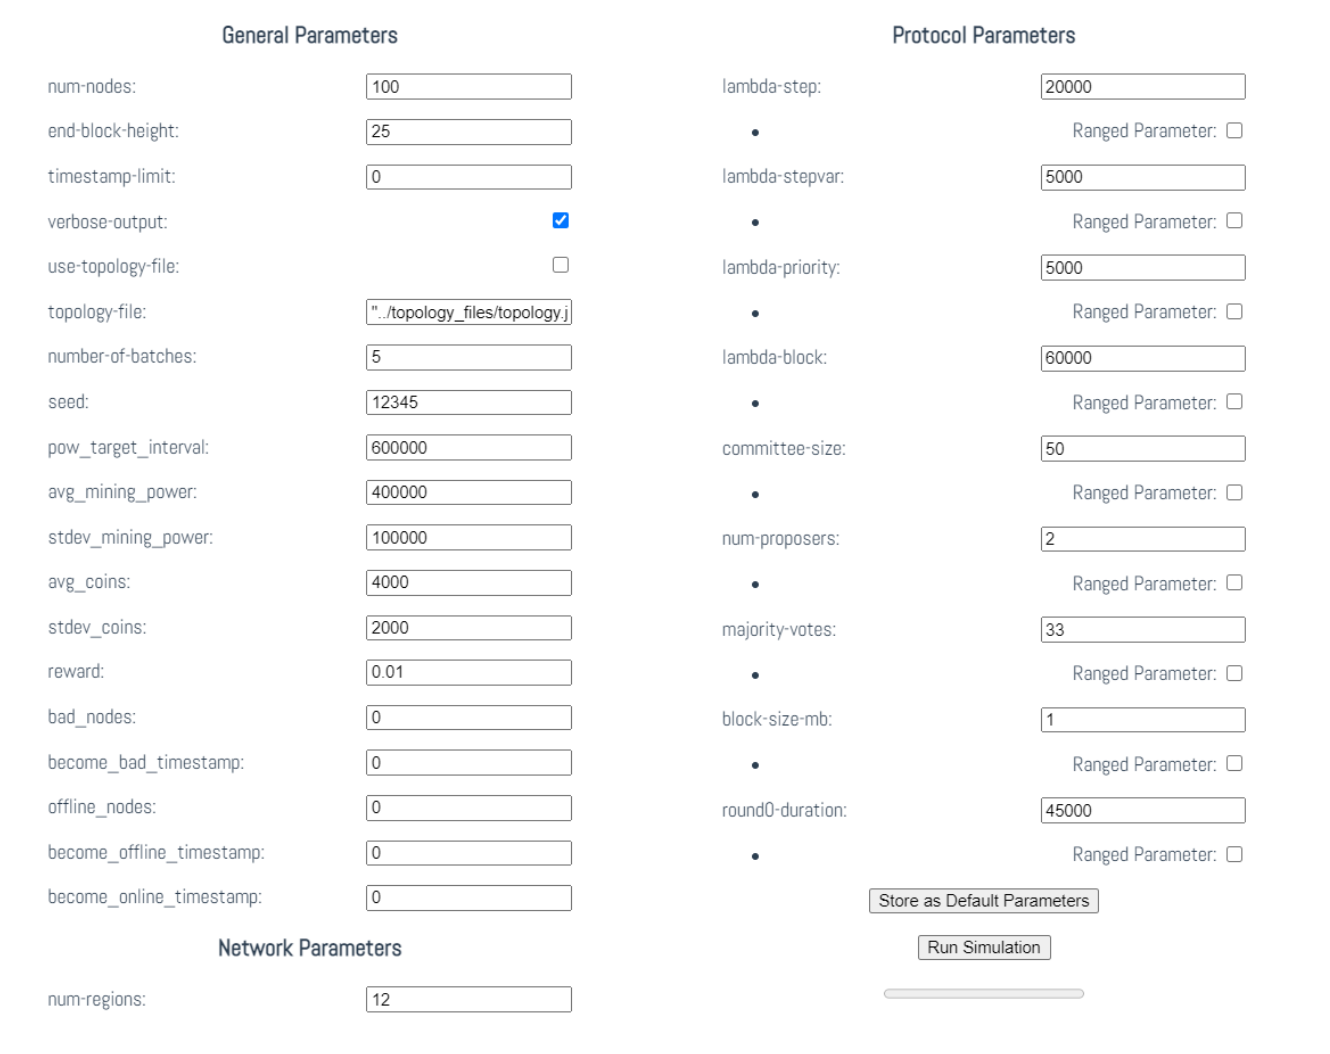
\includegraphics[width=4.5in, angle =0]{mobs_parameters}
	\caption{Parameters window}
	\label{fig:mobs_parameters}
\end{figure}

The Parameters window parses the parameters.json file and produces a form
where the user can customize the values or ranges of values for every parameter.

\subsubsection{Topology Specification}
\label{subsubsec:topology_specification}

The GUI also allows user to specify the topology of the network without needing
to manually write the JSON file. The Topology window offers a canvas to construct a network
topology as well as set individual parameters for each node.

\begin{figure}[h]
	\centering
	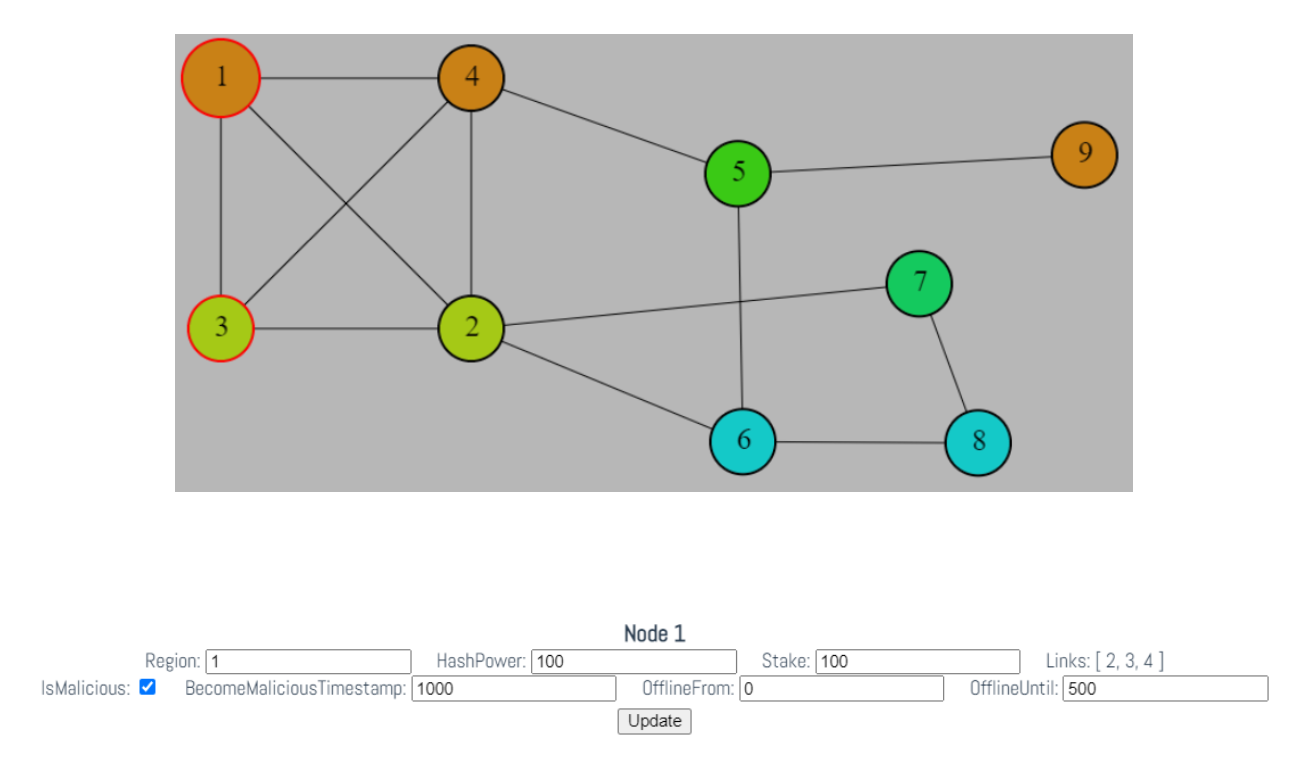
\includegraphics[width=4.5in, angle =0]{topology}
	\caption{Topology window and possible parametrizations for each individual node}
	\label{fig:topology}
\end{figure}

\subsubsection{Visualizer}
\label{subsubsec:visualizer}

\begin{figure}[h]
	\centering
	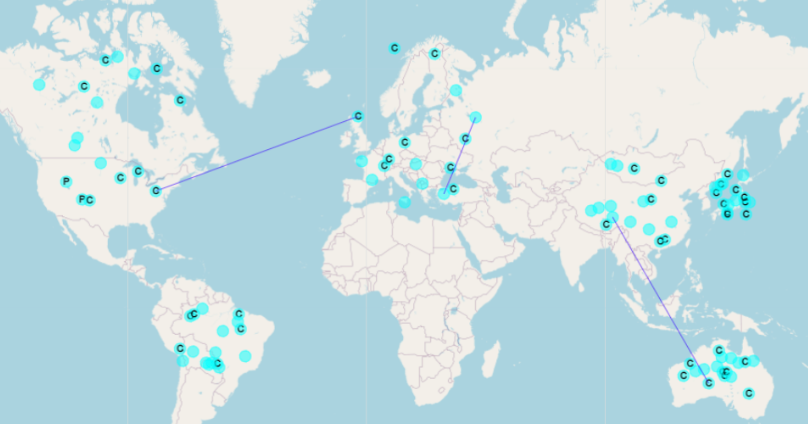
\includegraphics[width=4.5in, angle =0]{visualizer}
	\caption{Timelapse in the Visualizer window}
	\label{fig:visualizer}
\end{figure}

The Visualizer window allows user to play the state of each node in a time-lapse manner
and visualize exchanged messages.

\subsubsection{Statistical Analysis}
\label{subsubsec:statistical_analysis}

The Statistics window aids in the analysis of the metrics produced by the simulator.
The GUI will parse the output.json file and display it in an easy to read format.
These formats can come as graphs, displaying minimum and maximum values observed
for each metric that was produced and a graph with per node statistics.

\section{Critical Analysis}
\label{sub:membership_protocols}

In MOBs thesis we can see a detailed state-of-the-art study on other simulator
tools for Blockchain protocols. In this study it is noted that each of the tools
studied is mostly built with a specific purpose and not in being modular or extensible
to allow for the study of new scenarios and protocols,
nor in wide parametrization for different testing scenarios. The table bellow shows an
overview of the functionalities that each existing simulator and MOBs offer.

\begin{table}[h]
  \tiny
  \centering
  \begin{tabular}{|c|c|c|c|c|c|c|c|}
    \hline
    & \textbf{\begin{tabular}[c]{@{}c@{}}Adversarial\\ Behavior\end{tabular}} & \textbf{\begin{tabular}[c]{@{}c@{}}Offline \\ Nodes\end{tabular}} & \textbf{\begin{tabular}[c]{@{}c@{}}Bandwidth\\  Limits\end{tabular}}                      & \textbf{\begin{tabular}[c]{@{}c@{}}Network \\ Topology\end{tabular}}   & \textbf{Proof of Stake}                                   & \textbf{Proof of Work}                                                   & \textbf{GUI} \\ \hline
    \textbf{VIBES} \cite{vibes}   & yes                                                                     & \begin{tabular}[c]{@{}c@{}}not \\ modeled\end{tabular}            & \begin{tabular}[c]{@{}c@{}}not\\ modeled\end{tabular}                                     & \begin{tabular}[c]{@{}c@{}}generated \\ via \\ parameters\end{tabular} & \begin{tabular}[c]{@{}c@{}}not \\ modeled\end{tabular}    & bitcoin                                                                  & yes          \\ \hline
    \textbf{BlockSim} \cite{blocksim1} & \begin{tabular}[c]{@{}c@{}}not\\ modeled\end{tabular}                   & \begin{tabular}[c]{@{}c@{}}not \\ modeled\end{tabular}            & \begin{tabular}[c]{@{}c@{}}Throughput \\ calculated \\ from \\ distributionn\end{tabular} & \begin{tabular}[c]{@{}c@{}}fully \\ linked\end{tabular}                & \begin{tabular}[c]{@{}c@{}}not \\ modeled\end{tabular}    & \begin{tabular}[c]{@{}c@{}}bitcoin \\ ethereum\end{tabular}              & no           \\ \hline
    \textbf{BlockSim} \cite{blocksim2} & \begin{tabular}[c]{@{}c@{}}not\\ modeled\end{tabular}                   & \begin{tabular}[c]{@{}c@{}}not \\ modeled\end{tabular}            & \begin{tabular}[c]{@{}c@{}}not \\ modeled\end{tabular}                                    & \begin{tabular}[c]{@{}c@{}}fully \\ linked\end{tabular}                & \begin{tabular}[c]{@{}c@{}}not \\ modeled\end{tabular}    & \begin{tabular}[c]{@{}c@{}}bitcoin \\ ethereum\end{tabular}              & no           \\ \hline
    \textbf{SimBlock} \cite{simblock} & \begin{tabular}[c]{@{}c@{}}not \\ modeled\end{tabular}                  & \begin{tabular}[c]{@{}c@{}}not \\ modeled\end{tabular}            & \begin{tabular}[c]{@{}c@{}}specify \\ expected \\ available \\ bandwidth\end{tabular}     & \begin{tabular}[c]{@{}c@{}}generated \\ via \\ params\end{tabular}     & \begin{tabular}[c]{@{}c@{}}simple \\ example\end{tabular} & \begin{tabular}[c]{@{}c@{}}bitcoin \\ dogecoin \\ litecoin\end{tabular}  & yes          \\ \hline
    \textbf{MOBs}     & yes                                                                     & yes                                                               & parameterizable                                                                           & \begin{tabular}[c]{@{}c@{}}generated \\ via \\ params\end{tabular}     & tenderbake                                                & \begin{tabular}[c]{@{}c@{}}bitcoin \\ algorand \\ ouroboros\end{tabular} & yes          \\ \hline
    \end{tabular}
  \caption{Feature comparison between existing blockchain simulators and MOBS.}
  \label{table:1}
\end{table}

VIBES \cite{vibes}, is scalable, fast and capable of simulating Bitcoin-like
protocols however, there is a lack of separation between the code that defines the
simulator and the codes that defines the protocols, which makes implementing new
protocols difficult and time costly. On the GUI provided this lack of separation
also exists, having the statistics that are displayed tied to the protocols being
simulated, which means that if the user wants to implement a new protocol that has
different metrics/statistics, changes would need to be done to the GUI to support
them.

Neither BlockSim \cite{blocksim1}, BlockSim \cite{blocksim2} nor SimBlock \cite{simblock} 
support adversarial or byzantine behavior
of the nodes, making it impossible to test the protocols when the network is not in
perfect conditions.

VIBEs, BlockSim and BlockSim do not model Proof of Stake protocols which hinders
their extensibility, since as a result, these simulators don't offer abstractions
for timers and alarms commonly used in proof of stake.

MOBs addresses these concerns like described above offering a more modular and extensible
environment, an independent GUI and the ability to simulate different families of protocols.

\section{Initial Exercise}
\label{sub:initial_exercise}

As an initial exercise we chose to implement Chord in MOBs, this served twofold:

\begin{itemize}
  \item To understand how MOBs worked and how to use it to implement protocols
  \item To see the capabilities of MOBs in providing qualitative metrics to evaluate
a membership protocol.
\end{itemize}

To achieve this implementation we made use of MOBs Node module and implemented the
following events:

\begin{itemize}
  \item \textbf{Join: } An event that a node receives when another node first joins
the network. The receiving node will evaluate if the identifier of the new node makes him
a candidate to be that node's predecessor in the ring.
  \item \textbf{JoinResponse: } A node that has previously received a join will reply
with this event if the new node has been accepted as their predecessor. This contains
the identifier of the old predecessor so that the new node can make it its own.
  \item \textbf{Uft: } This event stands for update finger table, this event shares
an identifier known to a node, being from their finger table, their own, or one of
its neighbors with a random node. The receiver node will add this identifier to their finger table.
  \item \textbf{UpdateSuccessor: } This event is only used when a node updates their successor
this event is sent to itself as a way to log the new link.
  \item \textbf{UpdatePredecessor: } This event works the same way as UpdateSuccessor
but for the predecessor node.
  \item \textbf{RebalanceNetwork: } When a node receives this event it comes with
an identifier, the receiver node will see if the identifier is a better candidate for
their successor. This serves as a cyclic membership managing strategy.
  \item \textbf{SendRebalanceNetwork: } Periodically a node will propagate this message
to neighboring nodes to trigger a RebalanceNetwork event with their identifier.
\end{itemize}

The implementation of this protocol at the Node level turned out to not be successful.

One of the reasons is that when implementing this at the Node module, the network
module implements a network with a random graph, and as an initial operation, one
node would trigger a RebalanceNetwork with the identifier of another node and through
an epidemic broadcast fashion trigger all nodes into trying to join to other nodes.
This resulted in one of two scenarios:

\begin{itemize}
  \item Several Chord rings would be created instead of one single ring with all nodes,
making further communications since at the Chord protocol level, nodes from different rings
would be unknown from each other.
  \item After making nodes send periodic SendRebalanceNetwork events to neighboring
nodes at the Network module level, if the first couple of events made them unable to
integrate the ring they would become dormant, since the trigger to send  new
SendRebalanceNetwork events is triggered  by receiving events from other nodes
\end{itemize}

Another reason this protocol failed was that even leveraging overlay created at
the Network layer to send SendRebalanceNetwork events to know nodes at that level
to ensure that all nodes would converge to the same ring, this would create an enormous
amount of events that would slow down the simulator. This showed some promising results,
and we were able to see signs of a converging network, but the search for better neighbors
at the Chord level turned out to be a blind search, and the closer the network became to
converge the longer it took for new updates to take place.

To solve these issues we proposed move the implementation to the network module level.
This will make possible to initiate one node at a time and reduce blind lookups, solving
all three problems at once: 
\begin{itemize}
  \item Only one ring will be created
  \item Since nodes would always ping a known
member of the ring to join, the protocol would ensure they would be placed on the correct place
of the network and not be left out isolated
  \item Join operations in a formed chord ring would be less costly in the amount
of messages generated since we don't have to broadcast events and can instead target
to specific nodes.
\end{itemize}

We can also leverage this implementation at the network level to make the network
module even more modular and extensible, making it easier to implement new network protocols.
